\documentclass[11pt,a4paper]{article}
\usepackage[T1]{fontenc}
\usepackage[margin=2.3cm]{geometry}
\usepackage{amsmath,amssymb}
\usepackage{graphicx}
\usepackage[dvipsnames]{xcolor}
\usepackage{enumitem}
\usepackage[colorlinks=true,linkcolor=blue,urlcolor=blue]{hyperref}
\setlength{\parskip}{0.6em}
\setlength{\parindent}{0pt}
\begin{document}

\begin{center}{\LARGE\bfseries openregularity}\\[0.4em]{\large Learn what is known, and what is still unknown, about smooth fluid flow.}\\[0.2em]\small PAN IIT OSS explainer \textbullet{} higher secondary to diploma / undergraduate (levels 4-5)\end{center}

\section*{Why this exists}
Does a smooth fluid flow stay smooth for ever? For the 3-D Navier-Stokes equations nobody knows; it is a Clay Millennium Prize problem. This explainer teaches the question, what is known about it, and how to experiment on simple models without fooling yourself.

\section*{The end goal}
Learn what is known and unknown about smooth Navier-Stokes solutions (the Millennium problem). The end goal is to understand what is known and unknown about smooth Navier-Stokes solutions: a clear statement of the problem, the known 2-D and short-time results, the role of vortex stretching and the Beale-Kato-Majda criterion, and careful numerical practice. It does not claim or attempt a solution.

\section*{How the three sessions build up}
\begin{enumerate}[nosep]
\item \textbf{Session 1: Smooth or blow-up? The question and a toy} (Level 1, conceptual interactive model, 60 min).
\item \textbf{Session 2: Burgers: steepening against smoothing} (Level 2, mathematical engineering model, 75 min).
\item \textbf{Session 3: 2-D flow, 3-D vortex stretching, and numerical blow-up} (Level 3, simulation and validation, 90 min).
\end{enumerate}

\section{Session 1: Smooth or blow-up? The question and a toy}

\subsection*{A. Real-world problem}
Air in a room, water in a pipe and smoke from a candle are all described by the Navier-Stokes equations. Engineers solve them on computers every day. Yet one of the seven Clay Millennium Prize problems, stated by Fefferman, asks something very basic: if a 3-D flow of an ordinary fluid starts smooth, does it stay smooth for ever, or can its velocity gradient become infinite after a finite time? This is OPEN: nobody knows the answer, and this repo does not claim or attempt one. What we can do is understand what the question means and study toy models. How can a number that is finite now become infinite later at a definite time?

\subsection*{B. Concept and theory}
Navier-Stokes in plain words: the fluid velocity is carried along by itself (a nonlinear term) and smoothed by friction (viscosity). The question is whether the nonlinear steepening can ever beat the smoothing and produce infinite gradients in finite time. A toy for 'growth that feeds on itself' is dy/dt = y\textasciicircum{}p. For p = 2, separating variables gives y(t) = y0 / (1 - y0 t), which is infinite at t* = 1/y0; in general t* = 1/((p-1) y0\textasciicircum{}(p-1)) for p \textgreater{} 1. For p = 1 the solution y0 e\textasciicircum{}t is finite at every time. A second toy is the no-friction Burgers equation, where a sine wave steepens and its energy moves from one long wave to many short waves. Known results from the literature, in outline: Leray showed in the 1930s that weak (rough) solutions of 3-D Navier-Stokes exist for all time but without a proof that they are unique or smooth; local-in-time smooth solutions are known (work of Ladyzhenskaya, Kato and others); in 2-D smooth solutions exist for all time; the Beale-Kato-Majda criterion says a smooth solution can be continued as long as the time integral of the maximum vorticity stays finite. What is not known is global smoothness in 3-D.

\begin{itemize}[nosep]
\item y: a positive quantity that grows (toy) (arbitrary units)
\item y0: starting value of y (arbitrary units)
\item p: exponent in dy/dt = y\textasciicircum{}p (no unit)
\item t*: blow-up time (arbitrary units)
\item u: speed in the wave toy (arbitrary units)
\item k: wavenumber: number of waves in the box 2 pi long (no unit)
\end{itemize}

\begin{equation*}
\frac{dy}{dt}=y^{p}
\end{equation*}

\begin{equation*}
y(t)=\frac{y_0}{1-y_0 t}\quad(p=2),\qquad t^{*}=\frac{1}{y_0}
\end{equation*}

\begin{equation*}
t^{*}=\frac{1}{(p-1)\,y_0^{\,p-1}}\quad(p>1)
\end{equation*}

\begin{equation*}
u(x,t)=\sin X,\qquad x=X+t\sin X
\end{equation*}

\begin{center}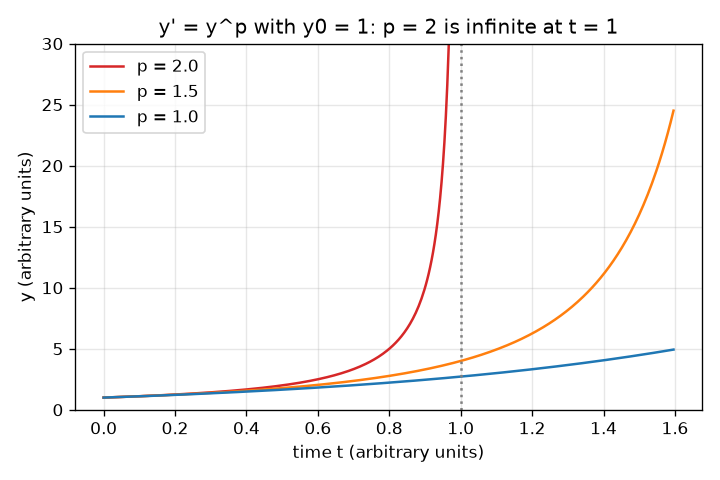
\includegraphics[width=0.85\linewidth]{figures/s01_blowup_vs_smooth.png}\\\small y' = y\textasciicircum{}p from y0 = 1: p = 2 and p = 1.5 blow up in finite time, p = 1 does not.\end{center}

\subsection*{E. Worked example}
For dy/dt = y\textasciicircum{}2 with y0 = 2, find the blow-up time and the value of y at t = 0.4. Check the blow-up time with a computer.
\begin{enumerate}[nosep]
\item Separate variables: dy / y\textasciicircum{}2 = dt, so -1/y = t - 1/y0 + ..., which gives y(t) = y0 / (1 - y0 t).
\item y is infinite when the denominator is zero: t* = 1/y0 = 1/2 = 0.5.
\item At t = 0.4: y = 2 / (1 - 2 * 0.4) = 2 / 0.2 = 10.
\item The computer (RK4 with steps that shrink as y grows) reaches y = 1,000,000 at t = 0.499999, which equals 0.5 - 1/y within 1e-5. The numbers agree.
\end{enumerate}
\textbf{Answer.} Blow-up at t* = 0.5; y(0.4) = 10.

\subsection*{F. Questions}
\begin{enumerate}[nosep]
\item \textbf{Conceptual.} In one or two sentences, what does the Navier-Stokes smoothness problem ask, and what is its status?
\item \textbf{Numerical.} For dy/dt = y\textasciicircum{}2, find the blow-up time for y0 = 4 and for y0 = 0.5. What happens to the time when y0 doubles?
\item \textbf{Graph and simulation interpretation.} On the growth view, which curve reaches the top of the plot first for y0 = 1: p = 2 or p = 1.5? What does p = 1 do?
\item \textbf{Design and optimisation challenge.} Design: you are told y follows dy/dt = y\textasciicircum{}2 and the model is only trusted until t = 1.5. Find the largest starting value y0 for which no blow-up occurs before t = 1.5, and one reason the answer is only a model result.
\end{enumerate}

\section{Session 2: Burgers: steepening against smoothing}

\subsection*{A. Real-world problem}
Traffic jams, breaking waves and sonic booms show smooth profiles turning into near-jumps. The 1-D Burgers equation u\_t + u u\_x = nu u\_xx is the simplest equation with this behaviour: the term u u\_x steepens, the term nu u\_xx smooths. It is NOT Navier-Stokes, but it is a clean laboratory for the competition between the two effects. For Burgers we can prove that solutions stay smooth for every nu \textgreater{} 0. How large does the gradient get as friction shrinks, and how fine must a computer grid be to see it? (Whether the 3-D Navier-Stokes equations always stay smooth is open.)

\subsection*{B. Concept and theory}
Without friction (nu = 0) each point keeps its speed, and the slope along it is u\_x = u0'/(1 + t u0'). It becomes infinite at the first time 1 + t u0' = 0, so t* = 1/max(-u0'). For u0 = sin x the steepest slope is -1 at x = pi, so t* = 1, and the slope at x = pi is -1/(1 - t). With friction, the Cole-Hopf substitution u = -2 nu d(ln phi)/dx turns Burgers into the heat equation phi\_t = nu phi\_xx, solved wave by wave: the solution is smooth for all t when nu \textgreater{} 0. Numerically we store u at N points, differentiate with Fourier waves, remove the top third of the waves (2/3 dealiasing, which avoids folding energy onto long waves) and step in time with RK4 and an integrating factor. Multiplying the equation by u and averaging over the box gives the energy equation dE/dt = -nu mean(u\_x\textasciicircum{}2), E = mean(u\textasciicircum{}2)/2: energy is lost only through gradients. The Reynolds number is the ratio of nonlinear to viscous effects; here Re = U L / nu = 1/nu with speed U = 1 and length L = 1.

\begin{itemize}[nosep]
\item u(x, t): speed (arbitrary units)
\item nu: viscosity (arbitrary units (length\textasciicircum{}2 / time))
\item t*: shock time without friction (time)
\item E: energy per unit length, mean(u\textasciicircum{}2)/2 (arbitrary units)
\item N: number of grid points (no unit)
\item P: peak gradient: maximum over time of max \textbar{}u\_x\textbar{} (1/time)
\item Re: Reynolds number 1/nu in these units (no unit)
\end{itemize}

\begin{equation*}
u_t+u\,u_x=\nu\,u_{xx}
\end{equation*}

\begin{equation*}
t^{*}=\frac{1}{\max_x\left(-u_0'(x)\right)},\qquad u_x=\frac{u_0'}{1+t\,u_0'}
\end{equation*}

\begin{equation*}
u=-2\nu\,\partial_x\ln\varphi,\qquad \varphi_t=\nu\,\varphi_{xx}
\end{equation*}

\begin{equation*}
\frac{dE}{dt}=-\nu\,\overline{u_x^{2}}
\end{equation*}

\begin{equation*}
P(\nu)=\max_t\max_x|u_x|\ \approx\ \frac{c}{\nu}
\end{equation*}

\begin{center}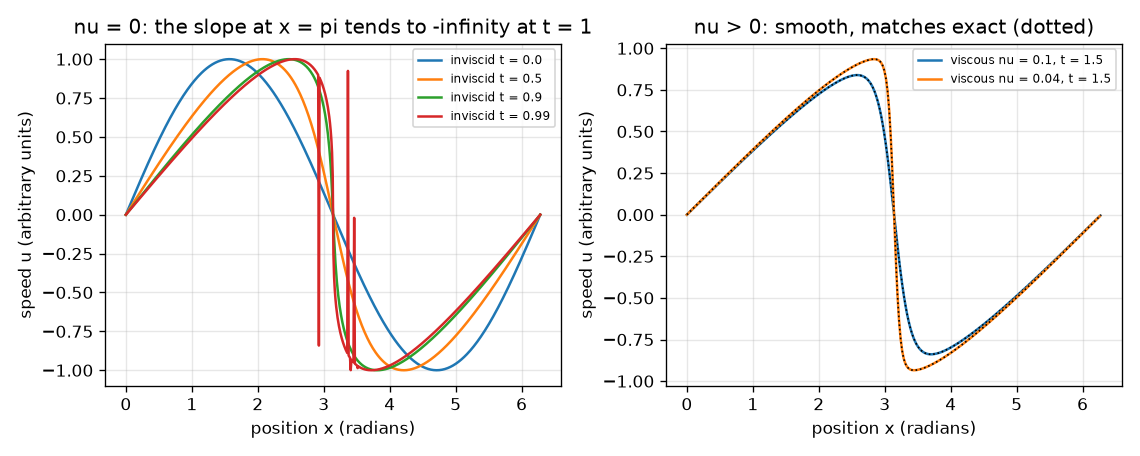
\includegraphics[width=0.85\linewidth]{figures/s02_burgers_profiles.png}\\\small No friction: the slope at x = pi tends to minus infinity at t = 1. With friction the solver (colour) lies on the exact solution (dotted).\end{center}

\subsection*{E. Worked example}
For u0 = sin x without friction, find the shock time and the slope at x = pi at t = 0.9. Then check numerically that with nu = 0.04 the viscous slope stays finite, with its steepest value -10.78 at t = 1.7.
\begin{enumerate}[nosep]
\item u0' = cos x, whose most negative value is -1 at x = pi, so t* = 1/1 = 1.
\item The slope at x = pi is u\_x = -1/(1 - t), so at t = 0.9 it is -1/0.1 = -10.
\item With nu = 0.04 the exact Cole-Hopf slope at x = pi and t = 1.7 is -10.78, and the spectral solver's peak gradient is the same number to 1e-4: the profile has a front but no infinity.
\item Check: the no-friction slope at t = 1.7 does not exist (shock formed at t = 1), while the viscous one is finite for every t.
\end{enumerate}
\textbf{Answer.} t* = 1; slope -10 at t = 0.9; with nu = 0.04 the largest slope is -10.78, reached around t = 1.7.

\subsection*{F. Questions}
\begin{enumerate}[nosep]
\item \textbf{Conceptual.} Why does the viscous Burgers solution stay smooth although the no-friction solution forms a shock?
\item \textbf{Numerical.} For u0 = 2 sin x without friction, find the shock time. How does it compare with u0 = sin x?
\item \textbf{Graph and simulation interpretation.} In the slope plot, which curve runs to minus infinity, and what does the viscous curve do for nu = 0.04? About when is it steepest?
\item \textbf{Design and optimisation challenge.} Design: a simulation of nu = 0.02 must have its peak gradient accurate to 1 percent. Using the convergence study, which power-of-two number of grid points do you need, what happens with half as many, and what about nu = 0.01?
\end{enumerate}

\section{Session 3: 2-D flow, 3-D vortex stretching, and numerical blow-up}

\subsection*{A. Real-world problem}
A weather map is nearly 2-D; the air behind an aircraft is 3-D. For 2-D flow we know that smooth solutions exist for all time. For 3-D flow we do not: the 3-D question is open and carries a Millennium Prize. What is different in 3-D? The vorticity (spin of the fluid) can be stretched by the flow, like a spinning ice skater pulling in their arms. This session shows the difference on a computer, without claiming anything about the open problem. It also asks a practical question: when a simulation 'blows up', is the equation singular or is the code under-resolved?

\subsection*{B. Concept and theory}
In 2-D the vorticity w = v\_x - u\_y is one number per point. With a stream function psi (u = psi\_y, v = -psi\_x), laplacian(psi) = -w and w\_t + u w\_x + v w\_y = nu laplacian(w). Vorticity is only carried and diffused; nothing stretches it. Consequences, for nu \textgreater{} 0 on a periodic box: the maximum of \textbar{}w\textbar{} cannot exceed its initial value (the exact statement is a maximum principle), energy obeys dE/dt = -2 nu Z, and enstrophy Z = mean(w\textasciicircum{}2)/2 obeys dZ/dt = -2 nu P with P = mean(\textbar{}grad w\textbar{}\textasciicircum{}2)/2 \textgreater{}= 0, so Z never grows. These facts are the reason 2-D global regularity is known. In 3-D the vorticity vector w = curl u obeys an equation with the extra term (w . grad) u = S w, where S is the strain (symmetric part of the velocity gradient). The number w . S w is positive where vortex lines are stretched. Nobody knows whether this term can drive a blow-up of smooth solutions; that is the open problem. Known 3-D results (from the literature): global weak solutions exist (Leray); smooth solutions exist for a short time (Ladyzhenskaya, Kato and others); the Beale-Kato-Majda criterion says a blow-up would require the time integral of the maximum vorticity to be infinite; Prodi-Serrin type conditions say smoothness persists if the velocity is controlled in certain norms; and Caffarelli-Kohn-Nirenberg proved that the possible singular set of suitable weak solutions is small. None of these settles the question. We implement 2-D with 2/3 dealiasing and RK4 with an integrating factor, and evaluate w . S w with spectral derivatives on the 3-D Taylor-Green field.

\begin{itemize}[nosep]
\item w: vorticity (spin) in 2-D (1/time)
\item u, v: velocity components (length/time)
\item psi: stream function (length\textasciicircum{}2/time)
\item nu: viscosity (length\textasciicircum{}2/time)
\item E: energy mean(u\textasciicircum{}2+v\textasciicircum{}2)/2 (length\textasciicircum{}2/time\textasciicircum{}2)
\item Z: enstrophy mean(w\textasciicircum{}2)/2 (1/time\textasciicircum{}2)
\item P: palinstrophy mean(\textbar{}grad w\textbar{}\textasciicircum{}2)/2 (1/(length\textasciicircum{}2 time\textasciicircum{}2))
\item k: wavenumber of the Taylor-Green flow (no unit)
\item S: strain tensor, symmetric part of grad u (1/time)
\end{itemize}

\begin{equation*}
w_t+u\,w_x+v\,w_y=\nu\,\Delta w,\qquad \Delta\psi=-w
\end{equation*}

\begin{equation*}
w(x,y,t)=2k\sin kx\,\sin ky\;e^{-2\nu k^{2}t}\quad\text{(Taylor-Green, exact)}
\end{equation*}

\begin{equation*}
\frac{dE}{dt}=-2\nu Z,\qquad \frac{dZ}{dt}=-2\nu P\le 0
\end{equation*}

\begin{equation*}
\partial_t\boldsymbol\omega+(\mathbf u\cdot\nabla)\boldsymbol\omega=(\boldsymbol\omega\cdot\nabla)\mathbf u+\nu\Delta\boldsymbol\omega,\qquad (\boldsymbol\omega\cdot\nabla)\mathbf u=S\boldsymbol\omega
\end{equation*}

\begin{equation*}
\int_0^{T}\|\boldsymbol\omega(t)\|_\infty\,dt<\infty\ \Rightarrow\ \text{smooth up to }T\quad\text{(Beale-Kato-Majda)}
\end{equation*}

\begin{center}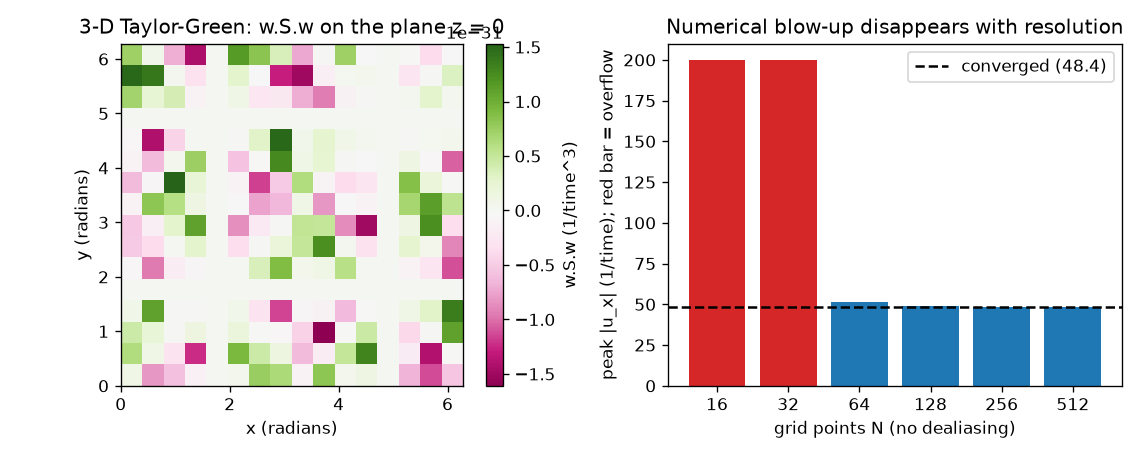
\includegraphics[width=0.85\linewidth]{figures/s03_stretching_and_artifact.png}\\\small 3-D Taylor-Green stretching term w . S w on one plane (left); Burgers peak gradient without dealiasing: coarse grids overflow, finer grids converge (right).\end{center}

\subsection*{E. Worked example}
Check the Taylor-Green solution with nu = 0.05 and k = 1 at t = 2: predict the maximum vorticity and the energy ratio E(2)/E(0), then compare with the solver.
\begin{enumerate}[nosep]
\item w0 = 2 sin x sin y has maximum 2. The exact decay factor is exp(-2 nu t) = exp(-0.2) = 0.8187.
\item So the maximum vorticity at t = 2 is 2 * 0.8187 = 1.637 (1/time).
\item Energy decays like exp(-4 nu t) = exp(-0.4) = 0.670, starting from E(0) = 0.25.
\item The solver on a 32 by 32 grid gives the same maximum and ratio; the largest pointwise difference from the exact field is about 1e-14. The nonlinear term vanishes identically for this flow, so only viscosity acts.
\end{enumerate}
\textbf{Answer.} Maximum vorticity 1.637 (1/time) and E(2)/E(0) = 0.670, matching the solver.

\subsection*{F. Questions}
\begin{enumerate}[nosep]
\item \textbf{Conceptual.} Why does 2-D vorticity have no stretching, and why does that help the regularity question there? Does this settle 3-D?
\item \textbf{Numerical.} For the Taylor-Green flow with k = 2, nu = 0.05, find the initial enstrophy and the decay factor of the vorticity at t = 0.5.
\item \textbf{Graph and simulation interpretation.} In the random 2-D run (nu = 0.01), the enstrophy drops from 0.356 to 0.185. What fraction is left, and what would a rise of the curve indicate?
\item \textbf{Design and optimisation challenge.} Design: you simulate Burgers with nu = 0.01 and see the solution overflow on a 32-point grid without dealiasing. List what you would change, in order, before claiming anything about singularities, and say what evidence would be convincing.
\end{enumerate}

\section{Real-world mini-project}
\textbf{How many Fourier modes does a thin front need?.} Choose the viscosity nu = 0.015. Use \texttt{convergence\_report} from Session 3 (or your own solver) to run the Burgers equation for u0 = sin x up to t = 3 on N = 32, 64, ..., 2048 points without looking at the exact answer. Report a table of N, the peak gradient (largest \textbar{}u\_x\textbar{} over time) and the change from one size to the next up. Declare the solution converged at the first N whose peak changes by less than 1 percent when N doubles. Then write three sentences explaining why a run that reports a smaller peak on a coarse grid is not evidence that the true gradient is small.

\section{The path ahead}
\begin{enumerate}[nosep]
\item \textbf{Session 4: A 3-D pseudo-spectral solver.} A 3-D periodic solver started from the 3-D Taylor-Green field.
\item \textbf{Session 5: Track the maximum vorticity.} A study of max \textbar{}w\textbar{}(t) for two or three 3-D initial fields, with the Beale-Kato-Majda integral.
\item \textbf{Session 6: Read about Euler blow-up claims and computer-assisted proofs.} A one-page reading summary that labels every claim as proved, supported by numerical evidence, or open.
\item \textbf{Session 7: Higher-precision Cole-Hopf.} A high-precision version of the exact Burgers solution.
\item \textbf{Session 8: A cheaper resolution.} A variant of the Burgers solver that places points where the front is.
\end{enumerate}

\section{Answers and hints}

\subsection*{Session 1}
\begin{enumerate}[nosep]
\item \textbf{Conceptual.} Hint: Think about initial data that is smooth, time, and a gradient becoming infinite. Is it solved? Solution: It asks whether, for smooth starting data, a 3-D incompressible viscous flow always has a smooth solution for all later times, or whether some quantity such as the velocity gradient can become infinite in finite time. It is an open Clay Millennium Prize problem: neither answer has been proved.
\item \textbf{Numerical.} Hint: Use t* = 1/y0. Solution: t* = 1/4 = 0.25 for y0 = 4 and t* = 1/0.5 = 2 for y0 = 0.5. Doubling y0 halves the blow-up time. Units: same time unit as t.
\item \textbf{Graph and simulation interpretation.} Hint: Compare t* = 1 with t* = 2. Solution: p = 2 blows up at t = 1 and p = 1.5 at t = 2, so p = 2 is first. For p = 1 the curve is the exponential e\textasciicircum{}t, which keeps growing but is finite at every t: fast growth is not the same as blow-up.
\item \textbf{Design and optimisation challenge.} Hint: You need t* = 1/y0 to be at least 1.5. Solution: 1/y0 \textgreater{}= 1.5 gives y0 \textless{}= 0.667 (2/3). Reason it is only a model: real systems have physics left out that would stop the growth earlier or change it, and y0 would be known only to some accuracy, so a safety margin is needed.
\end{enumerate}

\subsection*{Session 2}
\begin{enumerate}[nosep]
\item \textbf{Conceptual.} Hint: Compare the terms u u\_x and nu u\_xx when the gradient is very large. Solution: When the gradient is large the viscous term nu u\_xx grows too and spreads the front over a width of order nu. With nu \textgreater{} 0 the Cole-Hopf transform gives the heat equation, whose solutions are smooth, so the front stays thin but smooth. This is a statement about Burgers; it is not a proof for 3-D Navier-Stokes.
\item \textbf{Numerical.} Hint: Find the most negative value of u0' = 2 cos x. Solution: max(-u0') = 2, so t* = 1/2 = 0.5, half the time for sin x, because the profile is twice as steep.
\item \textbf{Graph and simulation interpretation.} Hint: Look at the grey curve and at the highest point of the viscous one. Solution: The grey no-friction curve -1/(1 - t) goes to minus infinity at t = 1. The viscous curve (nu = 0.04) reaches a minimum near -10.8 around t = 1.7 and then rises again as friction wins. Units: 1/time.
\item \textbf{Design and optimisation challenge.} Hint: Compare the errors for N = 256 and N = 512. Solution: N = 512: with N = 256 the error is about 1.7 percent (too large); with N = 512 it is below 0.2 percent. For nu = 0.01 you need N = 1024 (N = 512 gives about 1.9 percent). The needed N doubles when nu halves, because the front width scales with nu. Trade-off: the cost per step also rises and the time step must shrink.
\end{enumerate}

\subsection*{Session 3}
\begin{enumerate}[nosep]
\item \textbf{Conceptual.} Hint: In 2-D the vorticity points out of the plane and velocity does not vary along that direction. Solution: In 2-D the vorticity vector is perpendicular to the plane and the velocity has no component or variation along that direction, so (w . grad) u = 0. Vorticity is only carried and diffused, which gives the maximum principle and the enstrophy bound, and global smoothness is known. In 3-D the stretching term is present and global smoothness is not known; the problem is open, so nothing here settles it.
\item \textbf{Numerical.} Hint: Z0 = k\textasciicircum{}2/2 and the factor is exp(-2 nu k\textasciicircum{}2 t). Solution: Z0 = 4/2 = 2 (1/time\textasciicircum{}2). Factor = exp(-2 * 0.05 * 4 * 0.5) = exp(-0.2) = 0.819. The solver reproduces this decay to 1e-10 in the checkpoint.
\item \textbf{Graph and simulation interpretation.} Hint: Divide the two numbers; recall dZ/dt = -2 nu P with P at least 0. Solution: 0.185/0.356 = 0.52, so 52 percent is left. A rise would contradict dZ/dt \textless{}= 0 for 2-D flow: it would signal a bug, a time step that is too large, or missing resolution.
\item \textbf{Design and optimisation challenge.} Hint: Think of resolution, dealiasing, time step, and comparing several grids. Solution: First add dealiasing (the 2/3 rule) and check the time step; then repeat on N = 64, 128, 256, 512 and 1024 and watch the peak gradient converge: without dealiasing the peaks are 51.1, 48.8 and 48.4 for N = 64, 128, 256, and with dealiasing and N = 1024 it is 48.4. Convincing evidence of a real singularity would need convergence under refinement of a growing quantity, error bounds, and ideally a computer-assisted proof. Here the true solution is smooth for every nu \textgreater{} 0, so the overflow was purely numerical. Trade-off: more resolution costs more computing.
\end{enumerate}

\section{How to join}
Read \texttt{CONTRIBUTING.md} in the repository, then pick an issue labelled \texttt{good first issue}. Repository: \url{https://github.com/KrunalPanchal1995/openregularity}

\end{document}
